% !Mode:: "TeX:UTF-8"
\chapter{行为级仿真,时序分析及性能验证}

通过前面几章,详细描述了整个分支预测框架的设计细节以及相对于第一版做出的改进。本章主要介绍如何从多个方面来评估设计带来的提升,首先介绍我们使用的评估环境、评估指标和评估程序,并解释我们选择这些的原因。之后通过对比第一版香山和第二版香山的实验结果进行统计对比,体现本文设计的有效性和带来的提升。

\section{开发工具与实验平台}

\subsection{Chisel}

Chisel (Constructing Hardware In a Scala Embedded Language) 是加州大学伯克利分校开发的一种开源硬件构造语言,它是一个建构在Scala语言之上的领域专用语言 (DSL, Domain-Specific Language),不同于硬件设计领域传统的Verilog语言,Chisel建立在Scala这门高级编程语言之上,它能够使用大量高级语言才有的特性,比如面向象编程和函数式编程的思想,能够从更高的抽象程度来描述硬件电路,实现更多Verilog难以完成的功能,极大的提高使用者的开发效率

\subsection{Verilator}

Verilator是一款开源免费的Verilog/System Verilog仿真器,可用于将Verilog代码转换成C++代码,在服务器上对硬件设计进行行为级仿真验证。相比于类似的VCS,由于它仿真的电路只有0和1两个状态,不同于VCS有0、1、X、Z四个状态,因此它仿真运行的速度会更快

\subsection{差分测试框架}

在开发过程中,由于硬件电路非常复杂且难以调试,因此香山团队开发了一套差分测试框架,即使用一个正确的指令级的模拟器 (NEMU) 和硬件设计同时运行,在指令提交时比较两者的寄存器堆中的值是否相同,来判断硬件设计中有没有出现功能性bug,一次来提高发现和定位问题的效率。当然由于分支预测的特殊性,一些非功能性的错误无法检测。

\section{验证环境与评估指标}


\section{评估结果分析}

\begin{figure}[htb]
	\centering
	\setlength\tabcolsep{3pt}  % 同一行中的图片间隔
	\vspace{5pt} % 图片上部的空白,如果太小的话,图片顶部会与正文内容十分接近
	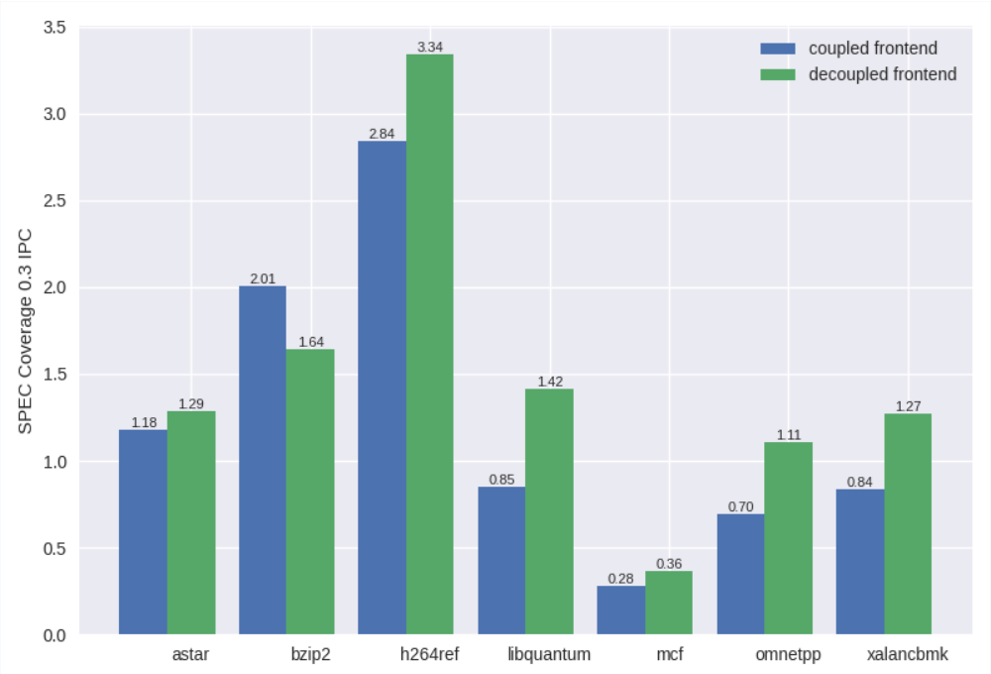
\includegraphics[width=0.7\textwidth]{spec2006_ipc.png}
	\caption{SPEC2006 coverage 0.8 部分检查点IPC对比}
	\label{fig:figure1}
\end{figure}

\begin{figure}[htb]
	\centering
	\setlength\tabcolsep{3pt}  % 同一行中的图片间隔
	\vspace{5pt} % 图片上部的空白,如果太小的话,图片顶部会与正文内容十分接近
	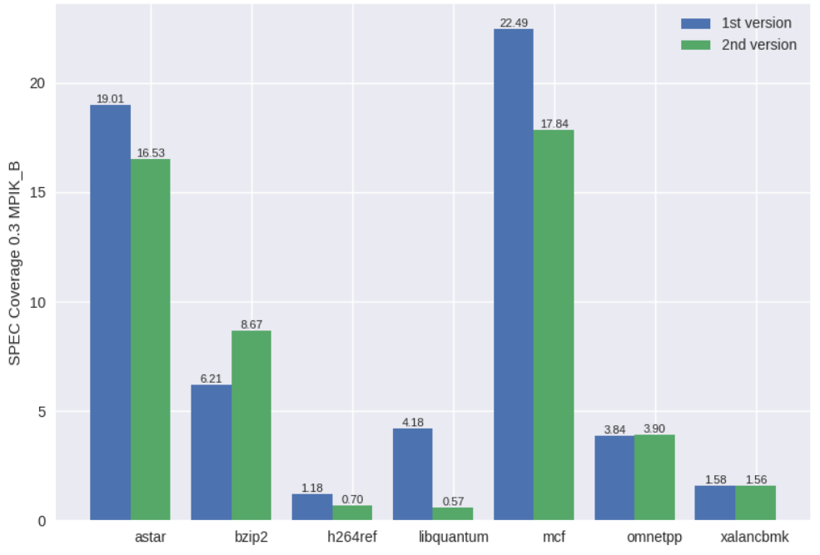
\includegraphics[width=0.7\textwidth]{spec2006_mpki.png}
	\caption{SPEC2006 coverage 0.8 部分检查点MPKI对比}
	\label{fig:figure2}
\end{figure}

% \begin{table}[]
%     \caption{两版架构频率对比}
%     \label{tb:table1}
%     \centering
%     \begin{tabular}{|c|c|c|}
%         \hline
%         版本   & 工艺   & 主频   \\ \hline
%         第一版 & 28nm & 1.3GHz \\ \hline
%         第一版 & 14nm & 1.8GHz \\ \hline
%         第二版 & 14nm & 2.0GHz \\ \hline
%     \end{tabular}
% \end{table}

\section{本章小结}

